% Extended abstract for the structural ray tracing work.
% Built with the ACM SIGGRAPH template (acmart, sigconf) in draft
% (nonacm) mode, since no venue-specific rights block applies yet.
%
% Compile with:  tectonic structural-rt-abstract.tex
% (or any TeX distribution that ships acmart).
\documentclass[sigconf,nonacm]{acmart}

\usepackage{listings}
\usepackage{xcolor}

% A minimal Slang language definition for listings.
\lstdefinelanguage{Slang}{
  morekeywords={struct,void,typealias,import,public,interface,
    associatedtype,float2,float3,uint,in,return},
  sensitive=true,
  morecomment=[l]{//},
  morestring=[b]",
}
\lstset{
  language=Slang,
  basicstyle=\scriptsize\ttfamily,
  keywordstyle=\bfseries\color[rgb]{0.10,0.25,0.55},
  commentstyle=\itshape\color[rgb]{0.30,0.45,0.30},
  columns=fullflexible,
  keepspaces=true,
  frame=single,
  framerule=0.3pt,
  xleftmargin=4pt,
  xrightmargin=2pt,
  aboveskip=6pt,
  belowskip=4pt,
  captionpos=b,
}

% Let TeX loosen lines slightly instead of overflowing into the margin
% (the narrow two-column measure plus unbreakable code tokens otherwise
% produces overfull lines).
\emergencystretch=8pt

\begin{document}

\title{Structural Ray Tracing: A Cross-Platform Slang Module for
Pipeline Ray Tracing}

\author{Kai Zhang}
\email{kazhang@nvidia.com}
\affiliation{%
  \institution{NVIDIA}
  \country{USA}% TODO: confirm city/country for the final submission.
}
% TODO: add co-authors/collaborators on the Slang team as appropriate.

\begin{abstract}
The Slang shading language compiles one shader codebase to all major
GPU APIs, yet pipeline ray tracing still cannot be written once and
compiled to every target: D3D12, Vulkan, and OptiX share a model of
free-standing stage entry points dispatched through a host-built shader
binding table (SBT), while Metal has no native \emph{miss} or
\emph{closesthit} stages and no complete SBT record indexing. On every API, a trace call's reachable
programs are invisible to the shader compiler, leaving that boundary
unchecked. We present \emph{structural ray tracing}, an experimental
Slang module in which the shader
declares a \emph{trace program schema} --- the finite, typed set of hit
groups, \emph{miss} shaders, and \emph{callable} shaders a trace can
reach --- while
the host retains full ownership of the physical SBT. The schema buys both portability and
compile-time checking: the compiler preserves native dispatch on D3D12,
Vulkan, and OptiX while synthesizing Metal's missing dispatch machinery,
and on every target it checks each trace call against its reachable
programs. For example, passing a payload type none of them expects
fails at compile time; on today's native APIs, the same mistake
surfaces only when the GPU misreads the payload at runtime. A Cornell-box demo runs one Slang
shader set on all of these APIs with output matching Slang's legacy
ray-tracing API, and a port of a Falcor~2--based renderer validates the
design
at mid-size-renderer scale.
\end{abstract}

\begin{CCSXML}
<ccs2012>
<concept>
<concept_id>10010147.10010371.10010382.10010385</concept_id>
<concept_desc>Computing methodologies~Ray tracing</concept_desc>
<concept_significance>500</concept_significance>
</concept>
<concept>
<concept_id>10011007.10011006.10011041</concept_id>
<concept_desc>Software and its engineering~Compilers</concept_desc>
<concept_significance>300</concept_significance>
</concept>
</ccs2012>
\end{CCSXML}
\ccsdesc[500]{Computing methodologies~Ray tracing}
\ccsdesc[300]{Software and its engineering~Compilers}

\keywords{ray tracing, shading languages, shader binding table, Slang,
Metal, Vulkan, DXR, OptiX, cross-platform GPU programming}

\maketitle

\section{Problem and Motivation}

Every native pipeline ray-tracing API couples three parties through
untyped conventions. The shader declares free-standing stage entry
points; the host builds an SBT whose records name those entry points and
carry per-record data; and a trace call selects records at runtime. On
D3D12, Vulkan, and OptiX the driver or hardware selects each hit-group
record through the same index calculation:
\begin{equation*}
\resizebox{\columnwidth}{!}{$
\underbrace{\mathit{recordIndex}}_{\text{driver/HW}} =
\underbrace{\mathit{instanceContribution}}_{\text{host, per instance}} +
\underbrace{\mathit{geometryIndex}}_{\text{host, per geometry}} \times
\underbrace{\mathit{sbtStride}}_{\text{trace call}} +
\underbrace{\mathit{sbtOffset}}_{\text{trace call}}
$}
\end{equation*}
A \emph{miss} record is instead selected directly by
$\mathit{missIndex}$, and a \emph{callable} record by the explicit index
passed to the call; the selected stages then dispatch natively.

Metal overlaps with only the traversal half of this model. During
traversal it does dispatch through a function table: each
\emph{candidate hit} --- a tentative intersection not yet accepted as
the closest --- can invoke a triangle or procedural intersection
function, Metal's \emph{anyhit}-style filter, selected by the sum of a
per-instance and a per-geometry table offset. But the trace call
contributes no $\mathit{sbtStride}$ or $\mathit{sbtOffset}$ analogue to
that index, the dispatched functions can only accept or reject their
candidate, and \emph{miss}, \emph{closesthit}, and \emph{callable} have
no stages at all: \emph{miss} and \emph{closesthit} logic is ordinary
control flow after \texttt{intersect()} returns, and a \emph{callable}
is an explicit function call the shader makes itself. Three concrete
gaps remain:

\begin{itemize}
\item \textbf{Dispatch-model gap.} No native dispatch reaches
  \emph{miss} or \emph{closesthit} code, and the traversal table index
  is not the full SBT
  record calculation: the trace-to-program mapping lives only in host
  pipeline setup.
\item \textbf{Resource mismatch.} Metal's function tables are
  shader-visible resources that must be declared and bound; the D3D12
  and Vulkan SBT has no shader-side binding point at all.
\item \textbf{Tag-inference gap.} Every reachable intersection function
  must carry a compatible \texttt{[[intersection(...)]]} tag
  list\footnote{Metal Shading Language Specification, version 4.1,
  \S2.17.1 (Ray-Tracing Intersection Tags), \S5.1.6 (Intersection
  Functions), and \S2.17.6 (Intersector Type): ``Intersection tags on
  the intersector type must match their associated intersection
  function \ldots\ or the behavior is undefined.''} --- the static
  signature of the traversal capabilities the function relies on and
  the inputs it may consume --- but reachability is host knowledge, so
  the compiler has no basis to infer those tag lists.
\end{itemize}

The practical consequence: engines either write and maintain their
pipeline ray-tracing shaders per platform, or skip Metal entirely. And
on every API, a trace call's reachable programs are invisible to the
shader compiler, so mistakes at that boundary are caught late --- if
ever.

\section{Technical Approach and Key Contributions}

The design rests on one ownership split. The \textbf{shader owns the
schema}: a trace program schema declares the finite set of executable
hit groups, \emph{miss} shaders, and \emph{callable} shaders, plus the
types of their
payloads, hit attributes, and per-record data. The \textbf{host owns the
SBT instance}: record count, order, program layout, and record bytes
remain runtime host decisions, exactly as in the native APIs. Stage
logic is written as stateless structs implementing stage interfaces
rather than free-standing entry points (Listing~\ref{lst:api}).

\begin{lstlisting}[float=tb,label={lst:api},caption={The new API surface.
A context fixes the payload, record, and primitive types; the schema
lists which programs exist; one typed descriptor binds the whole trace
program; the trace call is checked against the schema.}]
import slang.raytracing; // experimental module

struct RadianceHitContext : rt::IHitContext
{
    typealias TraceContext = SceneTraceContext;
    typealias Payload   = RadiancePayload;
    typealias Record    = MaterialRecord; // SBT record data
    typealias Primitive = rt::TrianglePrimitive;
}

struct RadianceClosestHit : rt::IClosestHitShader
{
    typealias Context = RadianceHitContext;
    void invoke(rt::ClosestHitInput<Context> input)
    {
        input.payload.radiance = shade(input.record,
            input.triangle.barycentricCoord);
    }
}

// The schema declares which programs exist -- not SBT records.
struct SceneSchema : rt::ITraceProgramSchema
{
    typealias TraceContext = SceneTraceContext;
    typealias HitGroups =
        rt::HitGroupList<RadianceGroup, ShadowGroup>;
    typealias MissShaders =
        rt::MissShaderList<SkyMiss, ShadowMiss>;
    typealias CallableShaders = rt::NoCallableShaders;
}

// One binding point for the whole trace program: on D3D12,
// Vulkan, and OptiX it lowers to no shader-visible resources;
// on Metal, to its function tables and record buffer.
rt::AccelerationStructure scene;
rt::TraceProgramDescriptor<SceneSchema> program;

// The payload type selects the matching programs in the schema.
rt::RayTracer<SceneSchema> tracer;
RadiancePayload p = {};
tracer.trace(desc, scene, program, p);
\end{lstlisting}

\textbf{Schema entries are code, not records.} A schema entry
identifies executable code --- it never claims a physical SBT record,
and no record index is assigned in shader source. The host still
decides record count, record order, and which program each record runs,
writing each record itself: one entry may back records 1, 4, and
10{,}000, each with different record data.

\textbf{Trace calls are no longer opaque.} Natively, the programs a
trace call may invoke are recorded only in host pipeline setup ---
invisible to the shader compiler. The schema gives each trace call a
deliberately weak, typed connection to its reachable hit-group,
\emph{miss}, and \emph{callable} programs: weak enough that the host
still owns record
placement, strong enough that mismatched payload and hit-attribute
types are diagnosed at compile time rather than at pipeline creation or
runtime, and that the reachable set stays visible while maintaining and
debugging a large ray-tracing codebase.

\textbf{One typed binding point.} The shader binds the whole trace
program as a single \texttt{TraceProgramDescriptor<Schema>}, closing
the resource mismatch: on D3D12, Vulkan, and OptiX the descriptor
lowers to no shader-visible resources --- the host builds the native
SBT exactly as today --- while on Metal the same declaration lowers to
the intersection-function tables, visible-function tables, and record
buffer that Metal requires, bound through reflection.

\textbf{Native where native exists, synthesized where it does not.} On
D3D12, Vulkan, and OptiX, stage structs lower to ordinary native entry
points and native SBT dispatch. On Metal, the same schema drives
synthesis of per-payload intersection-function-table dispatchers,
visible-function tables, a compiler-owned record buffer whose lookup
evaluates the standard hit-record index formula at runtime, and fully
inferred \texttt{[[intersection(...)]]} tag lists.

\textbf{Separate compilation.} A schema section may be left open, to be
completed at Slang link time by every linked type that implements a
designated tag interface --- so independently compiled modules (e.g.,
material plugins) contribute hit groups before final linking.

\textbf{A reflection contract.} From reflection, hosts read exact
target entry symbols, record layouts, the payload and hit-attribute
sizes pipeline creation requires, and more --- a single source of truth
for building each target's pipeline and SBT.

\section{Results and Demonstrations}

\begin{figure}
  \centering
  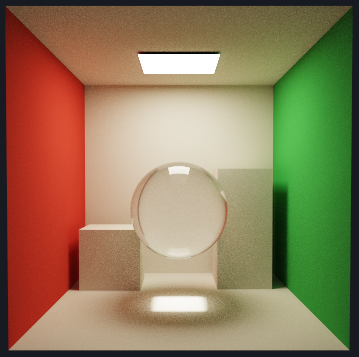
\includegraphics[width=0.52\columnwidth]{figures/cornell-demo.png}
  \caption{Cornell box path-traced through structural ray tracing
  (4096 samples per pixel, eight bounces): a procedural glass sphere
  --- a custom \emph{intersection} shader reporting custom hit
  attributes --- with refraction, floor caustics, and multi-bounce
  indirect lighting. One Slang shader set compiles unmodified to SPIR-V
  (Vulkan), DXIL (D3D12), OptiX/CUDA, and MSL (Metal).}
  \label{fig:cornell}
\end{figure}

A standalone Cornell-box demo (Figure~\ref{fig:cornell}) compiles one
Slang shader set unmodified to Vulkan and OptiX (Linux), D3D12
(Windows), and Metal (a direct Metal-cpp host consuming generated MSL
on macOS), and renders the same scene through the structural
ray-tracing API, Slang's legacy ray-tracing API --- the entry-point
path engines ship today --- and, on Metal, a hand-written native
implementation, with matching results on each backend. Early benchmarks
show no runtime cost --- expected by construction, since the structural
ray-tracing API introduces no code-generation difference from the
legacy one --- and its renders are byte-identical to the legacy API's
on the same backend. The one cost we do observe, as expected, is
compile time; exact figures await the final implementation.

The in-progress compiler implementation ($\sim$52K lines across 325
files) passes 401 dedicated compiler and runtime tests, and its runtime
suites pass on all of these backends --- including 16 native Metal
scenarios covering curves, motion, and multi-level acceleration
structures. A port of a Falcor~2--based renderer exercises
the design at mid-size-renderer scale: four ray-tracing consumers ---
including a reference path tracer whose schema serves two payload types
--- produce byte-identical output against the legacy ray-tracing API on
Vulkan, pass functional validation on both D3D12 and Vulkan, and
complete separate-compilation, reflection, and linking checks on
Metal.

\section{Limitations and What Attendees Will Learn}

This is work in progress. The design proposal is an open draft awaiting
review, and the implementation is not yet
merged;\footnote{Proposal: \url{https://github.com/shader-slang/spec/pull/59}.
Implementation: \url{https://github.com/shader-slang/slang/pull/12691}.
Cross-platform demo:
\url{https://github.com/kaizhangNV/structural-rt-cornell-demo}.}
the feature ships as an explicitly imported experimental module.
Version one covers pipeline ray tracing only --- inline ray queries are
already portable --- and excludes Shader Execution Reordering. The
Falcor~2 Metal runtime path awaits pipeline ray-tracing support in
Slang-RHI, and a port of Unreal Engine~5 is planned. The compiler
cannot validate host-written SBT contents --- the same trust boundary as
the native APIs, made explicit through reflection.

Attendees will learn why Metal breaks the SBT dispatch model that DXR,
Vulkan, and OptiX share; how declaring a typed schema in shader source
lets a compiler preserve native dispatch on three targets while
synthesizing it on Metal; what the compiler's trace checking can
and cannot guarantee; and how a reflection-driven host workflow replaces
per-platform SBT setup.

\end{document}
